\chapter{Statistical computation and software for dynamic quantile models}
\label{ch:research-a}

\section{Software contribution and scope}

The preceding chapter used extended dynamic quantile linear models to correct
and combine river-flow forecast products. That analysis also illustrates a
broader computational problem: dynamic quantile models require software that
connects state-space specification, posterior computation, diagnostics, and
forecasting without changing the inferential target between stages. The
\proglang{R} package \pkg{exdqlm} addresses this problem for Bayesian dynamic
and static quantile regression.

The statistical foundations precede the package. \citet{exd-yan2025family}
introduced the extended asymmetric Laplace (exAL) distribution and static
exAL regression. \citet{exd-me} developed the extended dynamic quantile
linear model (exDQLM), its original Markov chain Monte Carlo (MCMC) and
importance-sampling variational Bayes (ISVB) procedures, and a transfer-function
extension. The present contribution is the integrated software and subsequent
computation built around those methods. It consists of:
\begin{itemize}
\item a composable model-construction interface for trend, seasonal, regression, and transfer-function components in Bayesian dynamic quantile state-space models;
\item coordinated MCMC and variational interfaces, including scale-collapsed MCMC, ISVB, and a Laplace--delta variational Bayes (LDVB) procedure for dynamic and static fits;
\item fitted-model objects with standard functions for numerical summaries, plots, prediction, and diagnostics;
\item package-level exAL distribution utilities, predictive scoring and calibration diagnostics, and compiled implementations of computationally intensive model-building, posterior sampling and posterior predictive operations, with \proglang{R} fallbacks where applicable; and
\item static asymmetric Laplace (AL) and exAL regression with shrinkage priors, including the regularized horseshoe construction of \citet{exd-nishimura2023shrunken}, together with tests and replication materials for the reported analyses.
\end{itemize}

The \proglang{R} \citep{exd-R} software ecosystem for quantile regression is broad, but the capabilities most relevant to this chapter are distributed across software with different aims. Table \ref{exd:table:software} compares representative packages along four traits that are key to the scope of \pkg{exdqlm}: the primary modeling objective, the treatment of the temporal or latent-state structure, the inference strategy, and handling of multiple quantile levels.
The distinction between time included as an observed predictor and coefficients propagated as latent states is particularly important.
The computation column reports how fitting, posterior approximation, or state summaries are obtained, rather than treating these as additional model structures.
\begin{table}[h!]
\centering
\begingroup
\CompactTableStyle
\begin{tabularx}{\textwidth}{@{}l@{\hspace{0.7em}} >{\raggedright\arraybackslash}X >{\raggedright\arraybackslash}X >{\raggedright\arraybackslash}X >{\raggedright\arraybackslash}X@{}}
\toprule
\textbf{Package} & \textbf{Main scope} & \shortstack{\textbf{Temporal or}\\\textbf{state-space handling}} & \shortstack{\textbf{Inference or}\\\textbf{computation}} & \shortstack{\textbf{Multiple-quantile}\\\textbf{handling}} \\
\midrule
\pkg{quantreg} & General frequentist QR & Time-series regression formula: \code{dynrq()} handles lags, differences, trends, and seasons; no latent states & Optimization-based fitting; frequentist and bootstrap summaries & Vector-valued \code{tau}; post hoc rearrangement \\
\addlinespace[1pt]
\pkg{bayesQR} & Bayesian AL QR & Time or lags only as user-supplied covariates; no serial or state-space model & MCMC under the AL likelihood; optional adaptive lasso & Vector-valued quantiles; output by fitted quantile \\
\addlinespace[1pt]
\pkg{pqrBayes} & Bayesian penalized QR & Varying-coefficient regression: coefficients are B-spline functions of an observed modifier, possibly time; no serial or state-space model & MCMC with shrinkage priors & One target quantile per fit \\
\addlinespace[1pt]
\pkg{brms} & General Bayesian regression with an AL family & Regression autocorrelation terms can be added; no quantile state-space analysis sequence & Stan/NUTS posterior sampling & Fixed through the \code{asym\_laplace()} quantile parameter \\
\addlinespace[1pt]
\pkg{qgam} & Smooth additive QR & Time may enter as a smooth covariate; no serial or state-space model & Calibrated Gibbs posterior with GAM fitting & Single quantile via \code{qgam()}; multiple via \code{mqgam()} \\
\addlinespace[1pt]
\pkg{qrjoint} & Bayesian joint linear QR & Time only as a predictor; no serial or state-space model & Adaptive MCMC for joint quantile planes & Joint noncrossing quantile planes \\
\addlinespace[1pt]
\pkg{dlm} & Gaussian state-space modeling & Gaussian latent states with filtering, smoothing, and forecasting; not QR & Kalman state recursions; MLE or Bayesian parameter analysis & Not a quantile-regression package \\
\addlinespace[1pt]
\midrule
\pkg{exdqlm} & Bayesian exAL QR & Quantile latent states with filtering/smoothing summaries, forecasting, and transfer functions & MCMC posterior simulation; VB approximate posterior inference & Post hoc synthesis from separately fitted quantiles \\
\bottomrule
\end{tabularx}
\endgroup
\caption[Packages for quantile and state-space modeling]{\proglang{R} packages relevant to quantile and state-space modeling. Entries summarize documented primary interfaces along the dimensions used to position \pkg{exdqlm}; they are selective rather than exhaustive. In the temporal column, time-as-predictor/smooth/modifier uses, regression autocorrelation, Gaussian latent states, and quantile latent states are distinct categories. QR denotes quantile regression, AL asymmetric Laplace, exAL its extended version, NUTS the No-U-Turn sampler, GAM generalized additive model, MLE maximum likelihood estimation, and VB variational Bayes.}
\label{exd:table:software}
\end{table}


The principal distinction in Table~\ref{exd:table:software} is between time as
an observed predictor and coefficients evolving as latent states. The
\code{dynrq()} function in \pkg{quantreg} \citep{exd-quantreg} constructs
time-series regressions from lags, differences, trends, and seasonal terms, but
does not propagate coefficient states. Bayesian packages such as \pkg{bayesQR}
\citep{exd-bayesQR} and \pkg{pqrBayes} \citep{exd-pqrBayes} provide static AL
regression and shrinkage priors; the varying-coefficient formulation in
\pkg{pqrBayes} represents coefficients as spline functions of an observed
modifier rather than stochastic states. \pkg{brms} \citep{exd-brmsfamily}
supports AL regression within a broad Bayesian modeling system, while
\pkg{qgam}, \pkg{qrjoint}, \pkg{quantregGrowth}, and \pkg{qrcm} address
additive, joint, noncrossing, or coefficient-modeling objectives
\citep{exd-qgam,exd-qrjoint,exd-quantregGrowth,exd-qrcm}.

Conversely, general state-space packages such as \pkg{dlm} and \pkg{dynr}
provide Gaussian filtering and smoothing but not AL/exAL quantile likelihoods
or quantile-specific diagnostics and synthesis \citep{exd-dlm,exd-dynr}.
\pkg{exdqlm} therefore occupies a narrower position between general
quantile-regression and Gaussian state-space software. It is not intended to
replace software for broad static, additive, or joint multiquantile analysis.

The \code{exdqlm} package is distributed under the MIT License and is
available from the Comprehensive R Archive Network at
\url{https://CRAN.R-project.org/package=exdqlm}. The analyses reported below
use version 1.1.2, whose current interfaces include the structured LDVB
scale--skewness approximation, static shrinkage support, compiled computation,
diagnostics, and reproducibility checks used in this chapter. Chapter~\ref{ch:research-b} remains attached to
version 1.1.0, under which its hydrologic results were obtained. This distinction
preserves the statistical and computational provenance of both analyses rather
than treating package versions as interchangeable labels.

\section{Statistical models and posterior computation}
\label{exd:sec:exdqlm}

Chapter~\ref{ch:research-b} gives the complete dynamic formulation used in the
hydrologic application. A short statement here fixes the notation needed to
describe the software. Let \(p_0\in(0,1)\) be the target probability and let
\(\exAL_{p_0}(\mu,\sigma,\gamma)\) denote the exAL distribution with
\(p_0\)-quantile location \(\mu\), scale \(\sigma>0\), and admissible
skewness parameter \(\gamma\). Setting \(\gamma=0\) gives the AL special case.
For observations \(y_t\), the dynamic model is
\begin{align}
\label{exd:EQ:exDLM}
& \text{Observation equation:} & y_t &= \mat{F}_t^\top \vect{\theta}_t + \epsilon_t,  & \epsilon_t & \sim \exAL_{p_0}(0,\sigma,\gamma) \\
\label{exd:EQ:exDLMevo}
& \text{System equation:} & \vect{\theta}_t &= \mat{G}_t \vect{\theta}_{t-1} + \vect{\omega}_t, & \vect{\omega}_t  & \sim \N(\mat{0},\mat{W}_t).
\end{align}
Thus, \(\mat F_t^\top\vect\theta_t\) is the conditional
\(p_0\)-quantile. The design vector \(\mat F_t\), evolution matrix
\(\mat G_t\), and covariance \(\mat W_t\) may be assembled from trend,
seasonal, regression, and transfer-function components. Appendix
\ref{app:exdqlm-posterior} records the augmented posterior target used for
computation; the distributional derivation is not repeated here.

\subsection{Prior specification}
\label{exd:sec:priors}

The dynamic model assigns a normal prior to the initial state, an inverse-gamma
prior to \(\sigma\), and a proper Student-\(t\) prior to \(\gamma\), truncated
to its admissible interval \((L,U)\) \citep{exd-yan2025family}. Table
\ref{exd:table:priors} translates these statistical quantities into package
inputs. It is retained because it connects the model directly to the user
interface; the remaining prior algebra is given in Appendix
\ref{app:exdqlm-posterior}.

\begin{table}[!htb]
\centering
\TableStyle
\begin{tabular}{@{}lccccccccc@{}}
\toprule
\proglang{R} input & \multicolumn{4}{c}{\code{model}} & \multicolumn{2}{c}{\code{PriorSigma}}    & \multicolumn{3}{c}{\code{PriorGamma}}  \\
\cmidrule(lr){2-5}\cmidrule(lr){6-7}\cmidrule(l){8-10}
Mathematical symbol & $\mat{F}_{1:T}$ & $\mat{G}_{1:T}$ & $\mat{m}_0$ & $\mat{C}_0$ & $a_{\sigma}$ & $b_{\sigma}$ & $m_{\gamma}$ & $s_{\gamma}$ & $\nu_{\gamma}$ \\
\proglang{R} component & \code{FF} & \code{GG} & \code{m0} & \code{C0} & \code{a_sig} & \code{b_sig} & \code{m_gam} & \code{s_gam} & \code{df_gam} \\
Default if omitted & -- & -- & $\mat{0}_q$ & $10^3\mat{I}_q$ & 2.1 & 1.1 & 0 & 1 & 1 \\
\bottomrule
\end{tabular}
\caption[Translation from exDQLM notation to \pkg{exdqlm} inputs]{Translation from exDQLM notation to \pkg{exdqlm} inputs. The \code{model} object stores state-space components and the initial-state prior, while \code{PriorSigma} and \code{PriorGamma} store hyperparameters for $\sigma$ and $\gamma$. A dash indicates no generic default because \code{FF} and \code{GG} are determined by the selected model components. Here $\mat{0}_q$ and $\mat{I}_q$ denote a $q$-vector of zeros and the $q$-dimensional identity matrix.}
\label{exd:table:priors}
\end{table}
%%%%%%%%%%%%%%%%%%%%%%%%%%%%%%%%%%%%%%%%%
%%%%%%%%%%%%%%%%%%%%%%%%%%%%%%%%%%%%%%%%%
%%%%%%%%%%%%%%%%%%%%%%%%%%%%%%%%%%%%%%%%%

\subsection{Posterior computation}

The dynamic exDQLM posterior target and the original MCMC and ISVB inference strategy were developed by \citet{exd-me}. The package makes \code{exdqlmISVB()} available for variational inference following the ISVB approach of \citet{exd-me}.
The principal fitting routines are \code{exdqlmMCMC()}, which performs
posterior simulation, and \code{exdqlmLDVB()}, which implements the later
variational contribution studied in this chapter. The latter adapts the
nonconjugate variational strategy of \citet{exd-wang2013nonconjugatevb} to the
exAL scale--skewness block and couples it to Gaussian state smoothing.

The MCMC routine uses Gibbs sampling steps to update the latent-variable sequences
$\{s_t\}_{t=1}^T$ and $\{v_t\}_{t=1}^T$. The dynamic state sequence $\vect{\theta}_{1:T}$ is sampled using a forward-filtering backward-sampling algorithm \citep{exd-carter1994gibbs,exd-fruhwirth1994data}.
The scale and skewness parameters are updated separately from the latent-state blocks. By default, the package integrates $\sigma$ out of the conditional target for $\gamma$, updates $\gamma$ on its bounded logit scale using a univariate slice sampler \citep{exd-neal2003slice}, and then redraws $\sigma$ from its exact GIG conditional distribution. Joint
random-walk Metropolis--Hastings (MH) alternatives are also available.
The chain can optionally be initialized using the variational
approximation, but this initialization is separate from the subsequent MCMC
update kernel.


For longer time series or repeated model comparisons, MCMC can be computationally demanding. The \code{exdqlmLDVB()} routine uses blockwise coordinate-ascent variational inference. The blocks associated with the latent variables and dynamic states admit closed-form coordinate updates, whereas the scale--skewness block is nonconjugate. After \(\sigma\) and \(\gamma\) have been defined, the structured factorization can be stated unambiguously as \(q(\gamma)q(\sigma\mid\gamma)\): the marginal factor for \(\gamma\) is represented on its bounded logit scale, and the conditional factor for \(\sigma\) uses the generalized inverse Gaussian kernel available at each \(\gamma\). This conditional structure retains scale--skewness dependence that a fully factorized approximation would discard. The earlier two-dimensional Laplace--delta approximation on transformed \((\sigma,\gamma)\) coordinates remains available. The dynamic states are updated at each iteration using forward-filtering backward-smoothing, and convergence is monitored through changes in the state, scale, skewness, and evidence lower bound (ELBO).

Relative to the ISVB implementation, LDVB replaces the stochastic importance-sampling approximation for the non-conjugate scale--skewness block with a deterministic variational approximation conditional on the data and tuning inputs. This leads to reproducible convergence monitoring and provides approximate uncertainty summaries for both $\sigma$ and $\gamma$. After convergence, samples from the fitted variational factors are generated for posterior summarization. These are approximate variational draws rather than draws from the exact posterior, so MCMC remains the reference calculation when posterior tail behavior or interval accuracy is central.

The principal function-level controls are compact enough to state directly.
For \code{exdqlmMCMC()}, the defaults are the scale-collapsed slice kernel
\code{mh.proposal = "slice"}, 2000 burn-in iterations, and 1500 retained
draws. For \code{exdqlmLDVB()}, the default convergence tolerance is 0.1 and
the default number of requested variational draws is 200. The MCMC routine also
accepts \code{Sig.mh} as an optional proposal covariance when
\code{mh.proposal} selects a joint random-walk MH kernel; it is not used under
the default scale-collapsed slice update. Package-level options for compiled
and \proglang{R} implementation paths, including ELBO monitoring where applicable, are
described in Section~\ref{exd:sec:design} and are distinct from these
function-level controls.

%%%%%%%%%%%%%%%%%%%%%%%%%%%%%%%%%%%%%%%%%
%%%%%%%%%%%%%%%%%%%%%%%%%%%%%%%%%%%%%%%%%
%%%%%%%%%%%%%%%%%%%%%%%%%%%%%%%%%%%%%%%%%

\subsection{Evolution covariance and discount factors}
\label{exd:sec:dfs}

Both \code{exdqlmMCMC()} and \code{exdqlmLDVB()} use discount factors to specify the evolution covariance matrices $\mat{W}_t$ in Equation \eqref{exd:EQ:exDLMevo} \citep[see][and references therein]{exd-west1997bayesian,env-prado2021time}. Under a common discount factor $\delta \in (0,1],$ $\mat{W}_t = \frac{1-\delta}{\delta} \mat{G}_t \mat{C}_{t-1} \mat{G}_t^\top$ where $\mat{C}_{t-1}$ denotes the posterior variance of the state vector $\vect{\theta}_{t-1}$ at time $t-1$. The discount factor $\delta$ can be specified by the user via the function parameter \code{df}. The selection of discount factors can be done by optimizing a given selection criterion such as the continuous ranked probability score (CRPS) or the posterior predictive loss criterion (PPLC) defined in Section \ref{exd:sec:diags}, with Kullback--Leibler (KL) divergence as a complementary calibration diagnostic.  Discount factor selection is illustrated in Section \ref{exd:sec:ex2}.

Component-specific discounting is also available. When the state vector is partitioned into $h$ components with dimensions $q_1,\ldots,q_h$, each block of the evolution covariance matrix can be assigned its own discount factor.
The arguments \code{df} and \code{dim.df} specify the component discount factors $(\delta_1,\dots,\delta_h)$ and their corresponding dimensions $(q_1,\dots,q_h)$.  Section \ref{exd:sec:exs} provides examples.  \cite{exd-west1997bayesian} and \cite{env-prado2021time} give a detailed treatment of component discounting.

%%%%%%%%%%%%%%%%%%%%%%%%%%%%%%%%%%%%%%%%%
%%%%%%%%%%%%%%%%%%%%%%%%%%%%%%%%%%%%%%%%%
%%%%%%%%%%%%%%%%%%%%%%%%%%%%%%%%%%%%%%%%%

\subsection{Transfer-function models}
\label{exd:sec:tf}

Transfer functions provide a state-space representation for current and lagged input effects on a response quantile.
In \pkg{exdqlm}, this is handled by augmenting the dynamic state-space representation conditional on a fixed transfer-function rate \(\lambda\); both LDVB and MCMC routines fit the resulting model.
For input vector \(\mat x_t\), the augmented state contains an accumulated
effect \(\zeta_t\) and instantaneous coefficients \(\vect\psi_t\), with
\[
\zeta_t\mid\zeta_{t-1},\vect\psi_{t-1}
\sim\N\{\lambda\zeta_{t-1}+\mat x_t^\top\vect\psi_{t-1},\omega_t\},
\qquad 0<\lambda<1.
\]
The rate \(\lambda\) controls geometric decay of previous inputs, while
discount factors determine whether the instantaneous coefficients are fixed or
time-varying. The functions \code{exdqlmTransferMCMC()} and
\code{exdqlmTransferLDVB()} fit the augmented model. Appendix
\ref{app:exdqlm-posterior} gives the corresponding block evolution matrix;
function arguments and default priors are documented in the package reference
manual. The hydrologic analysis in Chapter~\ref{ch:research-b} provides the
principal dissertation application of external forecast inputs, although it
does not use this transfer-function example.

%%%%%%%%%%%%%%%%%%%%%%%%%%%%%%%%%%%%%%%%%
%%%%%%%%%%%%%%%%%%%%%%%%%%%%%%%%%%%%%%%%%
%%%%%%%%%%%%%%%%%%%%%%%%%%%%%%%%%%%%%%%%%

\subsection{Dynamic and static special cases}
\label{exd:sec:special}

Several commonly used models are special cases of the \code{exDQLM}. First, setting $\gamma=0$ reduces the exAL observation distribution to the AL distribution, i.e.,
$\epsilon_t \sim \exAL_{p_0}(0,\sigma,\gamma=0) = \AL_{p_0}(0,\sigma),$ leading to the dynamic quantile linear model (DQLM) of \cite{exd-gonccalves2017dynamic}. The DQLM can be implemented in \pkg{exdqlm} using the parameter \code{dqlm.ind = TRUE}.

Second, setting $\mat{G}_t=\mat{I}$ and $\mat{W}_t=\mat{0}$ reduces the model to the static exAL regression of \cite{exd-yan2025family}.
This model can be implemented using functions \code{exalStaticMCMC()} or \code{exalStaticLDVB()}.

Finally, combining these two restrictions gives static Bayesian linear quantile regression under the AL working likelihood \cite{env-yu2001bayesian}, as implemented in packages such as \pkg{bayesQR}. Within the \pkg{exdqlm} package, this model can be fitted using \code{exalStaticMCMC()} or \code{exalStaticLDVB()} with \code{al.ind = TRUE}, a static convenience alias for \code{dqlm.ind = TRUE}, which fixes $\gamma=0$.
Examples of these special models are given in Section \ref{exd:sec:exs}, with the sparse static regression analysis in Section \ref{exd:sec:ex4static}.

\subsection{Static exAL regression with shrinkage priors}
\label{exd:sec:static-model}

For independent observations \((y_i,\mat x_i)\), the static model replaces the
dynamic state by a regression coefficient vector:
\begin{equation}
y_i\mid\vect\beta,\sigma,\gamma
\sim\exAL_{p_0}(\mat x_i^\top\vect\beta,\sigma,\gamma),
\qquad i=1,\ldots,n.
\label{exd:eq:static-exal}
\end{equation}
The package supports Gaussian, lasso, horseshoe, and regularized horseshoe
priors. The Nishimura--Suchard regularized horseshoe option assigns each
nonintercept coefficient an effective prior precision
\(\tau^{-2}\lambda_j^{-2}+\zeta^{-2}\), where \(\tau\) is a global scale,
\(\lambda_j\) is a local scale, and \(\zeta\) bounds the variance of large
signals \citep{exd-nishimura2023shrunken}. Appendix
\ref{app:exdqlm-posterior} records the corresponding augmented update. Static
MCMC and LDVB are available through \code{exalStaticMCMC()} and
\code{exalStaticLDVB()}, respectively. This extension is statistically
distinct from the dynamic examples: it uses the same exAL likelihood and
scale--skewness computation but estimates fixed regression coefficients under
sparsity.

%%%%%%%%%%%%%%%%%%%%%%%%%%%%%%%%%%%%%%%%%
%%%%%%%%%%%%%%%%%%%%%%%%%%%%%%%%%%%%%%%%%
%%%%%%%%%%%%%%%%%%%%%%%%%%%%%%%%%%%%%%%%%
%%%%%%%%%%%%%%%%%%%%%%%%%%%%%%%%%%%%%%%%%
%%%%%%%%%%%%%%%%%%%%%%%%%%%%%%%%%%%%%%%%%
%%%%%%%%%%%%%%%%%%%%%%%%%%%%%%%%%%%%%%%%%

\subsection{Model diagnostics and forecasting}
\label{exd:sec:diags}


The package includes quantitative and graphical diagnostics for checking fitted quantile calibration, predictive performance, and forecasts.
Calibration is assessed using plug-in one-step-ahead probability integral transforms and standardized forecast errors. Predictive performance is summarized using CRPS and a target-quantile posterior-predictive loss criterion, while future quantiles and optional posterior-predictive draws are obtained through the standard \code{predict()} interface.

\subsubsection{Calibration diagnostics}
The one-step-ahead predictive probability integral transform (PIT) introduced by \cite{exd-rosenblatt1952remarks} is a useful diagnostic for models in which the marginal forecast distributions are not available in closed-form \citep{exd-huerta2003time,exd-prado2006multivariate}. Let $Y_t$ be the random response at time $t$ with observed value $y_t$ and let $y_{1:(t-1)}$ denote the observations available up to time $t-1.$ The one-step-ahead PIT is
\begin{align}
u_t^\star = \Pr(Y_t \leq y_t \mid y_{1:t-1}),
\label{exd:eq:pit_ideal}
\end{align}
 Under the true conditional distribution of $Y_t$
  given the past at every time, the PIT values $\{u_t^*\}$ are independent Uniform$(0,1)$ random variables \citep{exd-rosenblatt1952remarks}.

  The package reports a maximum a posteriori (MAP) plug-in version based on the conditional Gaussian filtering representation. If \(\hat f_t\) and \(\hat q_t\) denote the MAP plug-in one-step-ahead forecast location and variance, the stored standardized forecast error and the corresponding PIT diagnostic are
\begin{align}
\hat e_t =
\frac{y_t-\hat f_t}{\sqrt{\hat q_t}}, \;\;\; \text{and}
\label{exd:eq:standardized_error}
\;\;\;
\hat{u}_t = \Phi(\hat e_t),
\end{align}
where $\Phi$ denotes the standard normal CDF. These are diagnostic summaries of the fitted one-step-ahead sequence rather than posterior uncertainty bands for residuals.
Serial dependence in $\{\hat u_t\}$ is examined using an autocorrelation function (ACF) plot. The normal transformation $\Phi^{-1}(\hat{u}_t),$ which corresponds to $\hat{e}_t$ under the plug-in Gaussian representation, is assessed using a normal quantile--quantile (QQ) plot.

Departure from normality is also summarized using the KL divergence \citep{exd-kullback1951information}.
If $P_e$ denotes the density estimate of the MAP standardized forecast-error distribution and $\phi$ denotes the standard normal density, the package reports a forward diagnostic, denoted $\KL(P_e\,|| \ \phi)$ and, as a sensitivity measure, the reversed diagnostic $\KL(\phi \,||\,P_e)$.
Smaller values indicate closer marginal agreement with the plug-in standard
normal reference. This scalar diagnostic does not by itself establish complete
predictive calibration or independence of the PIT sequence.
These MAP standardized forecast errors are included in the output of the \code{exdqlmMCMC()} and \code{exdqlmLDVB()} functions.

\subsubsection{Predictive scoring}
The continuous ranked probability score (CRPS) evaluates the full posterior predictive distribution \citep{exd-gneiting2007}.
Let $\rho_p(x)=x[p-I(x<0)]$ denote the check loss at level $p$. For a predictive distribution $G$ and observation $y$, the CRPS is
\begin{equation}
\CRPS(y,G)=\mathbb{E}_{Y\sim G}|Y-y|-\frac{1}{2}\mathbb{E}_{Y,Y'\sim G}|Y-Y'|
=2\int_0^1 \rho_p\!\left(y-G^{-1}(p)\right)\,dp,
\label{exd:eq:crps_main}
\end{equation}
which shows that CRPS integrates check loss across all quantile levels and therefore evaluates the full predictive distribution rather than evaluating a single target level \(p_0\). In \code{diagnostics()}, posterior predictive draws define empirical quantiles \(\widehat q_t(\tau_k)\), giving the finite approximation
\begin{equation}
\widehat{\CRPS}_t
=
2\sum_{k=1}^{K} w_k
\rho_{\tau_k}\{y_t^{obs}-\widehat q_t(\tau_k)\},
\label{exd:eq:crps_iqs_main}
\end{equation}
where the weights \(w_k\) sum to one \citep{exd-laio2007verification}. The package uses the grid \(\tau_k=0.01,0.02,\ldots,0.99\) with equal weights and reports the CRPS values in \eqref{exd:eq:crps_iqs_main} averaged over time. A smaller value indicates better overall performance under this proper score; calibration and sharpness must be diagnosed separately. For a deterministic forecast, CRPS reduces to the absolute error, so its sample mean CRPS equals the mean absolute error (MAE).

Motivated by the posterior-predictive loss (PPL) framework of \cite{exd-gelfand1998model}, the package returns \code{pplc}, which evaluates the posterior predictive distribution under the target-level check loss $\rho_{p_0}$. That is,
\begin{align}
\PPLC = \sum_t \E[\rho_{p_0} (y_t^{obs}-y^{rep}_t) \mid y_{1:T}],
\label{exd:eq:pplc_main}
\end{align}
where the expectation is with respect to posterior predictive replicate draws generated from the observation equation \eqref{exd:EQ:exDLM} under posterior draws of the model parameters.
Smaller PPLC values indicate better performance.

Samples from the posterior replicate distributions are included in the output of \code{exdqlmMCMC()} and \code{exdqlmLDVB()}.

The function \code{diagnostics()} computes these calibration and predictive summaries for fitted dynamic objects. It returns an \code{exdqlmDiagnostic} object that can be summarized numerically or plotted.

\subsubsection{k-step-ahead forecasting}

For an arbitrary forecast origin \(\tilde t\), the conditional Gaussian
forecast distribution of the fitted quantile location is

\begin{equation}
\mat{F}_{\tilde{t}+k}^\top \vect{\theta}_{\tilde{t}+k}\mid y_{1:\tilde t}
\sim \N\!\left\{\mat{F}_{\tilde{t}+k}^\top \mat{a}_{\tilde{t}}(k),
\mat{F}_{\tilde{t}+k}^\top\mat{R}_{\tilde{t}}(k)\mat{F}_{\tilde{t}+k}\right\},
\label{exd:eq:forecast_recursion}
\end{equation}
where $\mat{a}_{\tilde{t}}(k) = \mat{G}_{\tilde{t}+k} \mat{a}_{\tilde{t}}(k-1)$, $\mat{R}_{\tilde{t}}(k) = \mat{G}_{\tilde{t}+k} \mat{R}_{\tilde{t}}(k-1) \mat{G}_{\tilde{t}+k}^\top + \mat{W}_{\tilde{t}+k}$, $\mat{a}_{\tilde{t}}(0) = \mat{m}_{\tilde{t}}$, and $\mat{R}_{\tilde{t}}(0) = \mat{C}_{\tilde{t}}$, with $\mat{m}_{\tilde{t}}$ and $\mat{C}_{\tilde{t}}$ denoting the filtered mean and covariance of $\vect{\theta}_{\tilde{t}}$, respectively. This distribution is implemented in the standard \code{predict()} method for fitted dynamic objects and is available for both MCMC and LDVB fits. The required inputs are a fitted object, a forecast origin \code{start.t}, and a positive horizon \code{k}. Future observation vectors \code{fFF} and evolution matrices \code{fGG} are supplied together when the forecast extends beyond stored model matrices. The credible mass \code{cr.percent} defaults to 0.95; posterior predictive draws are omitted by default and enabled with \code{return.draws}, with \code{n.samp} and \code{seed} controlling their number and reproducibility. The returned \code{exdqlmForecast} object contains forecast-quantile summaries and state moments, with posterior predictive draws included when requested. It can be plotted or evaluated against held-out observations using \code{diagnostics()}.


%%%%%%%%%%%%%%%%%%%%%%%%%%%%%%%%%%%%%%%%%
%%%%%%%%%%%%%%%%%%%%%%%%%%%%%%%%%%%%%%%%%
%%%%%%%%%%%%%%%%%%%%%%%%%%%%%%%%%%%%%%%%%
%%%%%%%%%%%%%%%%%%%%%%%%%%%%%%%%%%%%%%%%%
%%%%%%%%%%%%%%%%%%%%%%%%%%%%%%%%%%%%%%%%%
%%%%%%%%%%%%%%%%%%%%%%%%%%%%%%%%%%%%%%%%%

\section{Software design and numerical implementation}
\label{exd:sec:design}
\label{exdqlm:sec:body-inference}

The software separates statistical model specification from posterior
computation. Trend, seasonal, regression, and transfer components define a
state-space model that can be passed to MCMC or variational fitting procedures.
This separation makes comparisons between inferential methods meaningful:
the state equation and target quantile can be held fixed while the posterior
calculation changes.

Fitted dynamic and static models retain their inferential method and share a
common set of statistical operations. These operations provide state and
component summaries, fitted quantiles, forecasts, calibration diagnostics,
proper scores, and, when requested, posterior-predictive draws. Post-fit
synthesis combines predictive output from separately fitted quantile levels;
it does not convert those fits into a joint posterior over their parameters.
The examples below name individual functions only when the call clarifies the
statistical analysis. The complete function signatures, object classes, and
compatibility methods belong to the package reference documentation.

Computationally intensive density evaluation, Gaussian-state recursions,
latent-variable updates, and posterior-predictive simulation have
\proglang{C++} implementations through \pkg{Rcpp}, with corresponding
\proglang{R} implementations used for portability and numerical comparisons.
The selected computational implementation changes computation, not the statistical model. In version
1.1.2, the stochastic compiled paths used for the reported analyses obtain
their random-number streams from \proglang{R}; native numerical-library threads
are restricted in the recorded benchmarks so that timing and stochastic
variation have a stated reference condition.

The variational procedures record the evidence lower bound, scale, skewness,
and convergence summaries. Appendix~\ref{app:exdqlm-ldvb} describes the
closed-form, structured scale--skewness, and earlier Laplace--delta components,
together with the posterior blocks and numerical controls needed to interpret
them. The analyses reported here used \proglang{R} 4.6.0 and
\pkg{exdqlm} 1.1.2 on x86\_64 Linux, fixed random-number settings, and recorded
seeds. Reported run times are elapsed fitting times on that reference platform,
not machine-independent properties of the methods.

\section{Examples}
 \label{exd:sec:exs}


Two real-data analyses and one simulation benchmark examine statistically
distinct capabilities. Lake Huron examines dynamic model construction, MCMC
inference, forecasting, and posterior-predictive synthesis across separately
fitted quantiles. Sunspots examines component composition, LDVB inference,
diagnostics, discount-factor comparison, and comparison with MCMC. The
simulation then evaluates static exAL regression with a regularized horseshoe
prior and compares LDVB with MCMC.

The package also exposes distribution-level utilities for the exAL error family:
\code{dexal()}, \code{pexal()}, \code{qexal()}, and \code{rexal()} evaluate the
density, distribution function, quantile function, and random generator,
respectively, while \code{get\_gamma\_bounds()} returns the admissible interval
for $\gamma$ at a specified \(p_0\). These utilities support simulation, prior
calibration, and direct checks of the exAL distribution, but are not required
for the fitting, forecasting, diagnostic, or synthesis analyses below. CrI
denotes a credible interval in figure captions and plotting labels.

%%%%%%%%%%%%%%%%%%%%%%%%%%%%%%%%%%%%%%%%%
%%%%%%%%%%%%%%%%%%%%%%%%%%%%%%%%%%%%%%%%%
%%%%%%%%%%%%%%%%%%%%%%%%%%%%%%%%%%%%%%%%%

\subsection{Lake Huron}
\label{exd:sec:ex1}

The Lake Huron time series in \pkg{datasets} records annual lake levels (ft)
from 1875 to 1972. Figure \ref{exd:fig:ex1quants} reports the fitted dynamic
quantiles, forecast distributions, and synthesized predictive intervals. The
analysis also examines prior specification for $\gamma$ and MCMC computation
in a basic state-space model.

The analysis targets $p_0=0.95,0.50,$ and $0.05$. A second-order polynomial trend, constructed with \code{polytrendMod()}, defines the state-space structure and the prior quantities $\mat{F}_t,\mat{G}_t, \mat{m}_0$, and $\mat{C}_0$ from Section~\ref{exd:sec:exdqlm}. The initial level prior is centered at 579 ft, a rounded domain-scale value chosen before fitting rather than the sample mean, and the initial slope prior is centered at zero.


A discount factor of $0.9$ defines the evolution covariance matrix
$\mat{W}_t$. Section \ref{exd:sec:ex2} instead compares discount factors using
in-sample diagnostic criteria. The prior location parameters for \(\gamma\) are
quantile-specific: they are zero at the median and shifted in opposite
directions for the upper and lower tails, providing tail-specific
regularization within the admissible support. The scale parameter is 0.1 and
the number of degrees of freedom is 1. These quantities specify prior
information and do not determine the MCMC starting values. The reported fits
use \code{n.burn = 2000} and \code{n.mcmc = 3000}. Computation follows the
settings in Section \ref{exd:sec:design}; numerical and runtime provenance for
the recorded run is retained in the external replication logs.



The fitted object output is intentionally compact. It identifies the model
family, inference engine, quantile level, state dimension, retained posterior
draws, and the standard methods available for downstream analysis. The
\code{summary()} method adds draw dimensions and scalar posterior summaries.


By default, \code{exdqlmMCMC()} uses the package's LDVB routine,
\code{exdqlmLDVB()}, to warm-start the chain. This initialization choice is
separate from the subsequent MCMC kernel. The relative symmetry of the data
motivates a diagnostic fit to assess whether \(\gamma\) is far from zero at
\(p_0 = 0.5\). The unrestricted median model, denoted \code{M50.trace}, uses
7000 burn-in iterations and 3000 retained
draws. The stored trace and density summaries were inspected for both
parameters. Consistent with the symmetry of the data, the posterior mean of
\(\gamma\) is \(-0.004\) with a 95\% credible interval
\((-0.388, 0.475)\), while the posterior mean of \(\sigma\) is \(0.373\) with
a 95\% credible interval \((0.279, 0.461)\). Retained samples are \code{mcmc}
objects and remain available for more detailed diagnostics with \pkg{coda}
\citep{exd-coda}; a separate trace figure is not needed for the chapter's
substantive argument.



The unrestricted median run is used only to assess whether the additional
skewness parameter is needed at \(p_0=0.50\). This diagnostic run has a longer
burn-in because \(\gamma\) is sampled. Because its posterior is concentrated
near zero, the median model used in the quantile, forecast, and synthesis
panels is the fixed-\(\gamma\) DQLM \code{M50.dqlm}. Fixing \(\gamma\) removes
the skewness update from the MCMC kernel, so this fit uses the same 2000
burn-in iterations and 3000 retained draws as the other main fits. A
point-mass prior on $\gamma$ at 0 is specified by \code{gam.init = 0} and
\code{fix.gamma = TRUE}, equivalently \code{dqlm.ind = TRUE}. This
specification gives the DQLM described in Section \ref{exd:sec:special}.



The fitted \code{exdqlmMCMC} objects support subsequent analysis and forecasting. The top-left panel of Figure~\ref{exd:fig:ex1quants} shows posterior mean estimates and 95\% CrIs for the three dynamic quantiles. The fitted-object \code{plot()} method places the quantiles on common axes when \code{add = TRUE}.


\begin{figure}[!t]
\centering
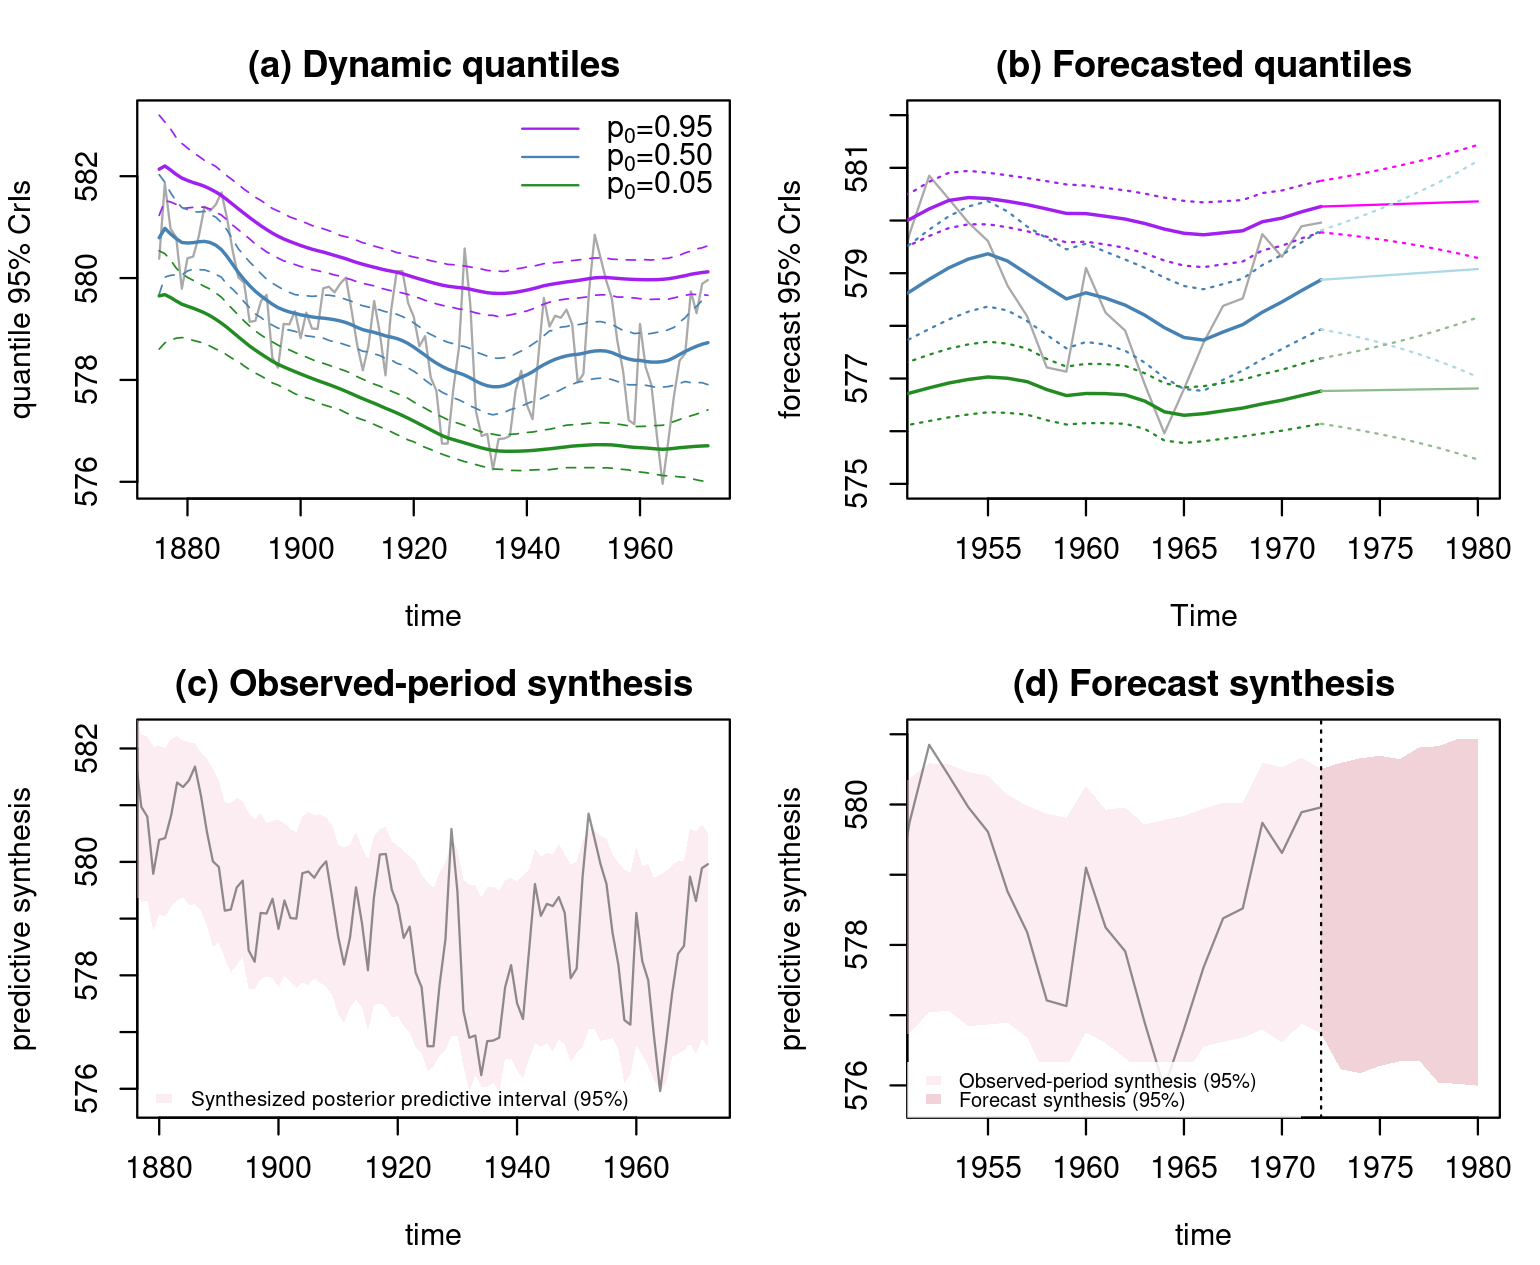
\includegraphics[width=0.9\textwidth]{figures/ch02-exdqlm/ex1quants.png}
\caption[Lake Huron dynamic quantile analysis]{Example 1: Lake Huron. Top-left: posterior mean estimates and 95\% CrIs of the estimated quantiles, plotted with the data (grey). Top-right: forecasted quantile estimates and 95\% credible intervals (seen after 1972), along with the filtered quantile estimates and 95\% credible intervals (seen from 1952 to 1972). Bottom-left: synthesized posterior predictive 95\% interval over the observed period. Bottom-right: observed-period synthesis near the forecast origin (lighter band) and synthesized posterior predictive 95\% interval over the eight-step forecast window (slightly darker rose band); the vertical dotted line marks the forecast origin.}
\label{exd:fig:ex1quants}
\end{figure}

The eight-step-ahead forecast distributions begin in 1972. Their updates use the observational vector \code{fFF} and evolution matrix \code{fGG}; both are time invariant and identical to those used for estimation.


The forecast objects are obtained with \code{predict()} at the final observed time, \code{start.t = length(LakeHuron)}, and are displayed on common axes with \code{plot()} and \code{add = TRUE}.



The top-right panel of Figure~\ref{exd:fig:ex1quants} shows the forecast quantile estimates and 95\% CrIs after 1972 together with the filtered estimates before 1972. The \code{cr.percent} argument controls the displayed credible level.

When several quantile models are fitted separately, the package also allows their posterior predictive draws to be combined into a single coherent predictive distribution through \code{quantileSynthesis()}. Each fitted model contributes local predictive information near its target quantile, and the synthesis step interpolates across these quantile-specific draws to obtain one posterior predictive distribution. When independently fitted quantiles induce crossing, optional monotonicity corrections based on isotonic adjustment and monotone rearrangement are available \citep{exd-barlow1972,exd-chernozhukov2010}. The synthesis operates on posterior predictive draws indexed by quantile level, so the input fits need not use identical skewness restrictions. For Lake Huron, it combines exDQLM tail fits at \(p_0=0.05\) and \(0.95\) with the fixed-\(\gamma\) DQLM median fit \code{M50.dqlm}.



The recorded run uses the package's default isotonic adjustment and monotone rearrangement. The stored synthesized quantile summaries have no remaining crossings over the observed period.

With \code{return.draws = TRUE}, each object stores posterior predictive
forecast draws in \code{samp.fore}. The same synthesis step can therefore be
applied over the eight-step forecast horizon.



The same correction settings are used for the forecast synthesis, and the eight-step synthesized forecast summaries are also ordered across the three input quantile levels.

The objects \code{syn.obs} and \code{syn.fore} have class \code{exdqlmSynthesis}, so the corresponding \code{plot()} method displays the synthesized posterior predictive intervals. The first synthesis panel in Figure~\ref{exd:fig:ex1quants} shows the observed-period interval. The second uses the same synthesis near the forecast origin, overlays the forecast synthesis, and shades the one-step bridge from the final observed interval to the first forecast interval.



%%%%%%%%%%%%%%%%%%%%%%%%%%%%%%%%%%%%%%%%%
%%%%%%%%%%%%%%%%%%%%%%%%%%%%%%%%%%%%%%%%%
%%%%%%%%%%%%%%%%%%%%%%%%%%%%%%%%%%%%%%%%%

\subsection{Sunspots}
\label{exd:sec:ex2}

The yearly Sunspot time series in \pkg{datasets} contains counts from 1700 to
1988 (Figure \ref{exd:fig:ex2quant}). Upper-tail sunspot activity provides an
example of dynamic quantile modeling for cyclic count data. The analysis
targets the \(0.85\) quantile with a continuous exAL working likelihood; it is
not a discrete-count likelihood analysis. It compares exDQLM and DQLM fits,
examines LDVB diagnostics, and uses those diagnostics to screen discount
factors. The state contains a first-order polynomial trend and a Fourier
seasonal component with an 11-year fundamental period and its first four
harmonics, for a total of 9 state parameters. The \pkg{exdqlm} functions accept
time-invariant \code{dlm} objects: \code{dlmModPoly()} constructs the trend
component, which \code{as.exdqlm()} converts to an \code{exdqlm} object.

The initial level prior is centered at 50 sunspots, a rounded count-scale value chosen before fitting, with prior standard deviation 50 to keep the level weakly informative on the observed count scale. The \code{seasMod()} function constructs the seasonal component with the first four Fourier harmonics of the approximately 11-year sunspot cycle.

Adding the trend and seasonal \code{exdqlm} objects produces a block-composed
state-space model with one trend state and eight seasonal states. The
component-specific discount factors are $0.9$ for the trend component of
dimension $1$ and $0.85$ for the seasonal component of dimension $8$, specified by
\code{df = c(0.9, 0.85)} and \code{dim.df = c(1, 8)}.

\begin{figure}[t]
\centering
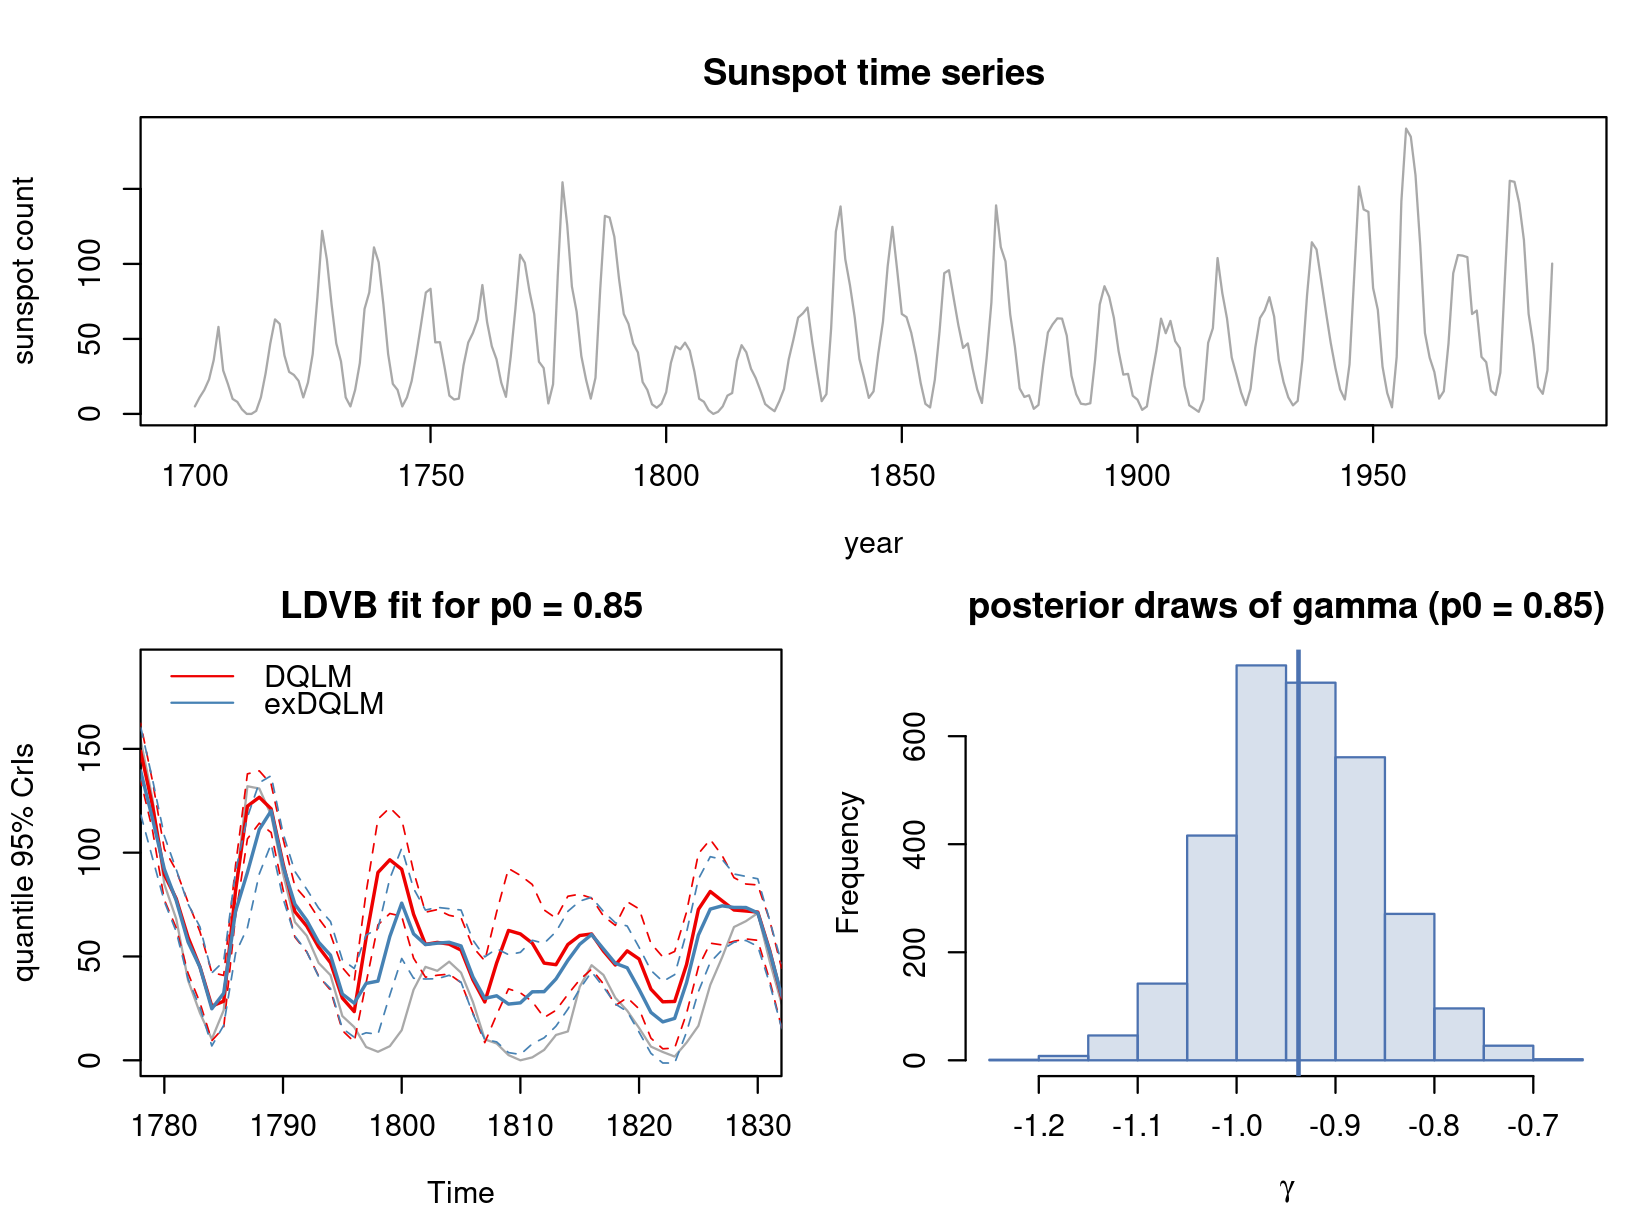
\includegraphics[width=1\textwidth]{figures/ch02-exdqlm/ex2quant.png}
\caption[Sunspots DQLM and exDQLM comparison]{Example 2: Sunspots. Top: The sunspot time series from 1700 to 1988. Bottom left: posterior mean estimates and 95\% CrIs of the estimated quantiles from the DQLM (red) and exDQLM (blue), plotted with the data (grey) from 1780 to 1830. Bottom right: Histogram of samples from the approximated posterior distribution of $\gamma$ under the exDQLM.}
\label{exd:fig:ex2quant}
\end{figure}

The LDVB approximations are obtained with \code{exdqlmLDVB()}. Setting
\code{dqlm.ind = TRUE} gives the DQLM, whereas the default specification gives
the exDQLM. Both fits use \code{sig.init = 2} as the starting value for the
LDVB scale update and \code{n.samp = 3000}.



The fitted objects can be summarized with the \code{summary()} generic, which reports the model class, sample size, state dimension, discount factors, convergence iterations, and run time. For this dataset of length 289, the DQLM LDVB fit completes more quickly, while the corresponding exDQLM LDVB fit is more computationally demanding because the skewness parameter is estimated rather than fixed. The timing comparison in Table \ref{exd:tab:ex2bench} reports the values from the recorded benchmark setting. These runtimes are fit elapsed times stored in the returned fit objects; they are intended for within-setting comparison and should not be interpreted as machine-independent timing constants.

The lower-left panel of Figure~\ref{exd:fig:ex2quant} compares the two fitted dynamic quantiles over 1780--1830 using the fitted-object \code{plot()} method.



\begin{figure}[t]
\centering
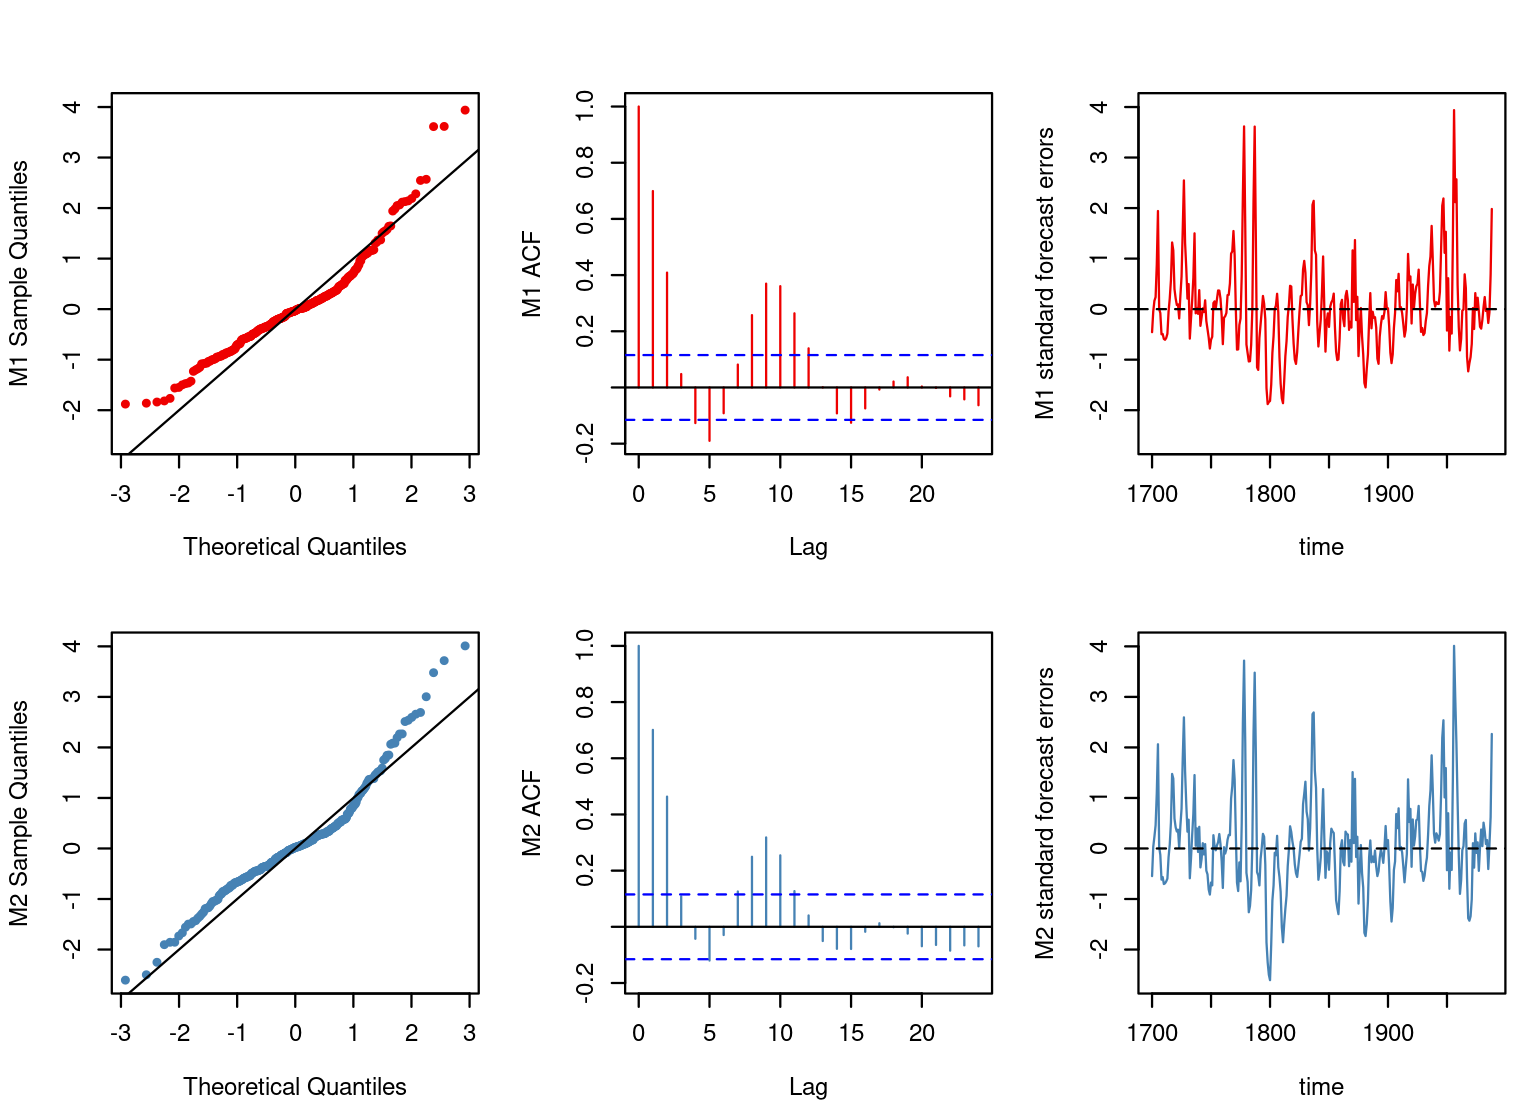
\includegraphics[width=1\textwidth]{figures/ch02-exdqlm/ex2checks.png}
\caption[Sunspots calibration diagnostics]{Example 2: Sunspots. The QQ plots (left column), ACF plots of the PIT sequence (center column), and MAP one-step-ahead standardized forecast errors (right column) from the DQLM (red) and exDQLM (blue).}
\label{exd:fig:ex2checks}
\end{figure}

The approximate posterior distribution of $\gamma$ assesses whether the
exDQLM's additional skewness flexibility is supported by the fitted
approximation. Figure \ref{exd:fig:ex2quant} plots samples from the
corresponding variational distribution. Its mass lies away from zero for this
upper-quantile fit.



The \code{diagnostics()} method returns an \code{exdqlmDiagnostic} object whose
\code{plot()} method produces Figure \ref{exd:fig:ex2checks}. The plots use
the MAP one-step-ahead standardized forecast errors from the filtering
recursion and the corresponding probability integral transform (PIT)
sequence. They therefore summarize fitted diagnostic sequences rather than
posterior bands for residuals.



The \code{diagnostics()} method also supports a coarse in-sample comparison of
candidate model specifications. A grid of seasonal discount factors is fitted
with LDVB and compared through the resulting CRPS and KL values. Because the
criteria use the same observations that fit each model, the comparison is a
diagnostic screen rather than an out-of-sample predictive validation. CRPS is
the primary criterion and KL divergence is a complementary calibration check;
the selected specification has the smallest CRPS.


On this coarse grid, the CRPS and KL criteria agree and both select the seasonal discount factor \(0.85\), so the choice used above is retained.

Matched DQLM and exDQLM specifications fitted with \code{exdqlmMCMC()} provide
the posterior-simulation comparison. They use the same state-space model,
quantile level, and discount factors as the LDVB fits, with 2000 burn-in
iterations and 3000 retained draws.



\begin{table}[t!]
\centering
\TableStyle
\begin{tabular}{@{}llrrrr@{}}
 \toprule
 model & method & \shortstack{runtime\\(s)} & KL & CRPS & PPLC \\
 \midrule
 \tworowcell{DQLM} & LDVB & \textbf{22.53} & \textbf{0.133} & 8.525 & 3851.4 \\
 & MCMC & 125.48 & 0.170 & \textbf{7.580} & \textbf{2966.0} \\
 \midrule
 \tworowcell{exDQLM} & LDVB & \textbf{73.46} & \textbf{0.107} & 6.558 & 3015.2 \\
 & MCMC & 174.66 & 0.212 & \textbf{5.120} & \textbf{2206.8} \\
 \bottomrule
\end{tabular}
\caption[Sunspots dynamic benchmark]{Example 2: representative dynamic benchmark for the DQLM and exDQLM fits at \(p_0 = 0.85\). Each row reports fit runtime together with the deterministic KL normality diagnostic, the mean CRPS from posterior predictive empirical quantiles, and the posterior predictive loss criterion (PPLC). The LDVB rows use \code{n.samp = 3000}. The MCMC rows use 2000 burn-in iterations and 3000 retained draws. Runtimes are fit elapsed times stored in the returned fit objects and exclude diagnostic calculations, plotting, table construction, and document rendering. They were measured under benchmark setting B on an Intel Xeon E5-4650 CPU with \proglang{R} 4.6.0, \pkg{exdqlm} version 1.1.2, the C++ MCMC implementation in \code{"fast"} mode, and \code{exdqlm.cpp\_threads = 1L}. Because the columns are the comparison metrics, bold entries indicate the smaller value within each model block; displayed ties are left unbolded.}
\label{exd:tab:ex2bench}
\end{table}

Table~\ref{exd:tab:ex2bench} gives the runtime-and-diagnostic comparison.



Within each model class, LDVB is substantially faster. For both DQLM and exDQLM, LDVB gives the smaller KL value, while MCMC gives smaller CRPS and PPLC values. Comparing model classes within each inferential method, the exDQLM improves the LDVB diagnostics relative to the DQLM, and under MCMC it improves the predictive-score criteria CRPS and PPLC. The comparison shows why runtime is reported together with predictive criteria rather than by itself.

%%%%%%%%%%%%%%%%%%%%%%%%%%%%%%%%%%%%%%%%%
%%%%%%%%%%%%%%%%%%%%%%%%%%%%%%%%%%%%%%%%%
%%%%%%%%%%%%%%%%%%%%%%%%%%%%%%%%%%%%%%%%%

\paragraph{Transfer-function capability.}
The package also fits dynamic models with current and geometrically decaying
input effects through the transfer-function routines described in Section
\ref{exd:sec:tf}. A separate Big Tree water-flow example and its full
replication record remain in the software article and package materials
\citep{env-deleon2026exdqlm}. It is not repeated here because
Chapter~\ref{ch:research-b} gives the dissertation's substantive river-flow
analysis. This choice keeps the present examples focused on capabilities not
already covered in the preceding chapter.

\subsection{Sparse static exAL regression benchmark}
\label{exd:sec:ex4static}


The static routines are evaluated under a correlated Gaussian regression
benchmark for which the target conditional quantile is known exactly. Let
\[
\mat{x}_i \sim \N_8(\mat{0}, \Sigma_x),\qquad (\Sigma_x)_{jk} = 0.5^{|j-k|},
\]
with sparse signal
\[
\vect{\beta}^\star = (3,\,1.5,\,0,\,0,\,2,\,0,\,0,\,0)^\top.
\]
For each target quantile level \(p_0\), the data-generating mechanism is
\[
Y_i^{(p_0)} = \mat{x}_i^\top \vect{\beta}^\star + \sigma_\varepsilon \{Z_i - \Phi^{-1}(p_0)\},
\qquad Z_i \sim \N(0,1),\qquad \sigma_\varepsilon = 1.5.
\]
Then
\[
Q_Y(p_0 \mid \mat{x}_i) = \mat{x}_i^\top \vect{\beta}^\star,
\]
so the true \(p_0\)-quantile is the same sparse linear signal at each fitted quantile level. Note that this is a quantile-specific calibration benchmark: each target level is generated so that the known target quantile is the same sparse linear signal, rather than a single-response multi-quantile analysis. The Gaussian data-generating distribution does not coincide with the exAL working likelihood; the benchmark therefore evaluates recovery of a correctly specified conditional quantile under likelihood misspecification. Gaussian design matrices are generated with \code{MASS::mvrnorm()} from \pkg{MASS} \citep{exd-MASS}.
The design uses \(n = 160\) training observations and an independent holdout
sample of size \(800\).



Separate static exAL models are fitted at
\(p_0 \in \{0.05,0.25,0.50\}\). All fits use the Nishimura--Suchard
regularized horseshoe prior \citep{exd-nishimura2023shrunken}, implemented as
\code{beta_prior = "rhs\_ns"}, with \(\tau_0 = 0.15\), fixed slab
\(\zeta^2 = 9\), and an unshrunk intercept. The LDVB fit uses
\code{exalStaticLDVB()} with \code{n.samp = 3000}; the MCMC fit uses
\code{exalStaticMCMC()} with \code{n.burn = 2000} and
\code{n.mcmc = 3000}. The MCMC routine uses its default
\code{collapsed\_slice} scale--skewness kernel and is warm-started from LDVB.
The lower-tail LDVB fit at \(p_0 = 0.05\) converges more slowly and therefore
has a larger iteration budget. Setting \code{al.ind = TRUE}, equivalently
\code{dqlm.ind = TRUE}, would recover the AL special case in Section
\ref{exd:sec:exdqlm}; the reported analysis instead uses the general static
exAL model with sparse \code{rhs\_ns} shrinkage.



For static fits, the \code{diagnostics()} method summarizes fitted quantiles on a common design matrix and, when holdout responses or a reference quantile are supplied, reports predictive evaluation metrics such as check loss and reference-quantile error. It also stores posterior coefficient summaries that can be plotted with \code{plot(..., type = "coefficients")}. In this simulated example, the true coefficient vector is known, so Figure \ref{exd:fig:ex4static} overlays it as a visual reference. This truth overlay is optional through the parameter \code{beta.ref} and is not needed for real data applications.



\begin{figure}[!t]
\centering
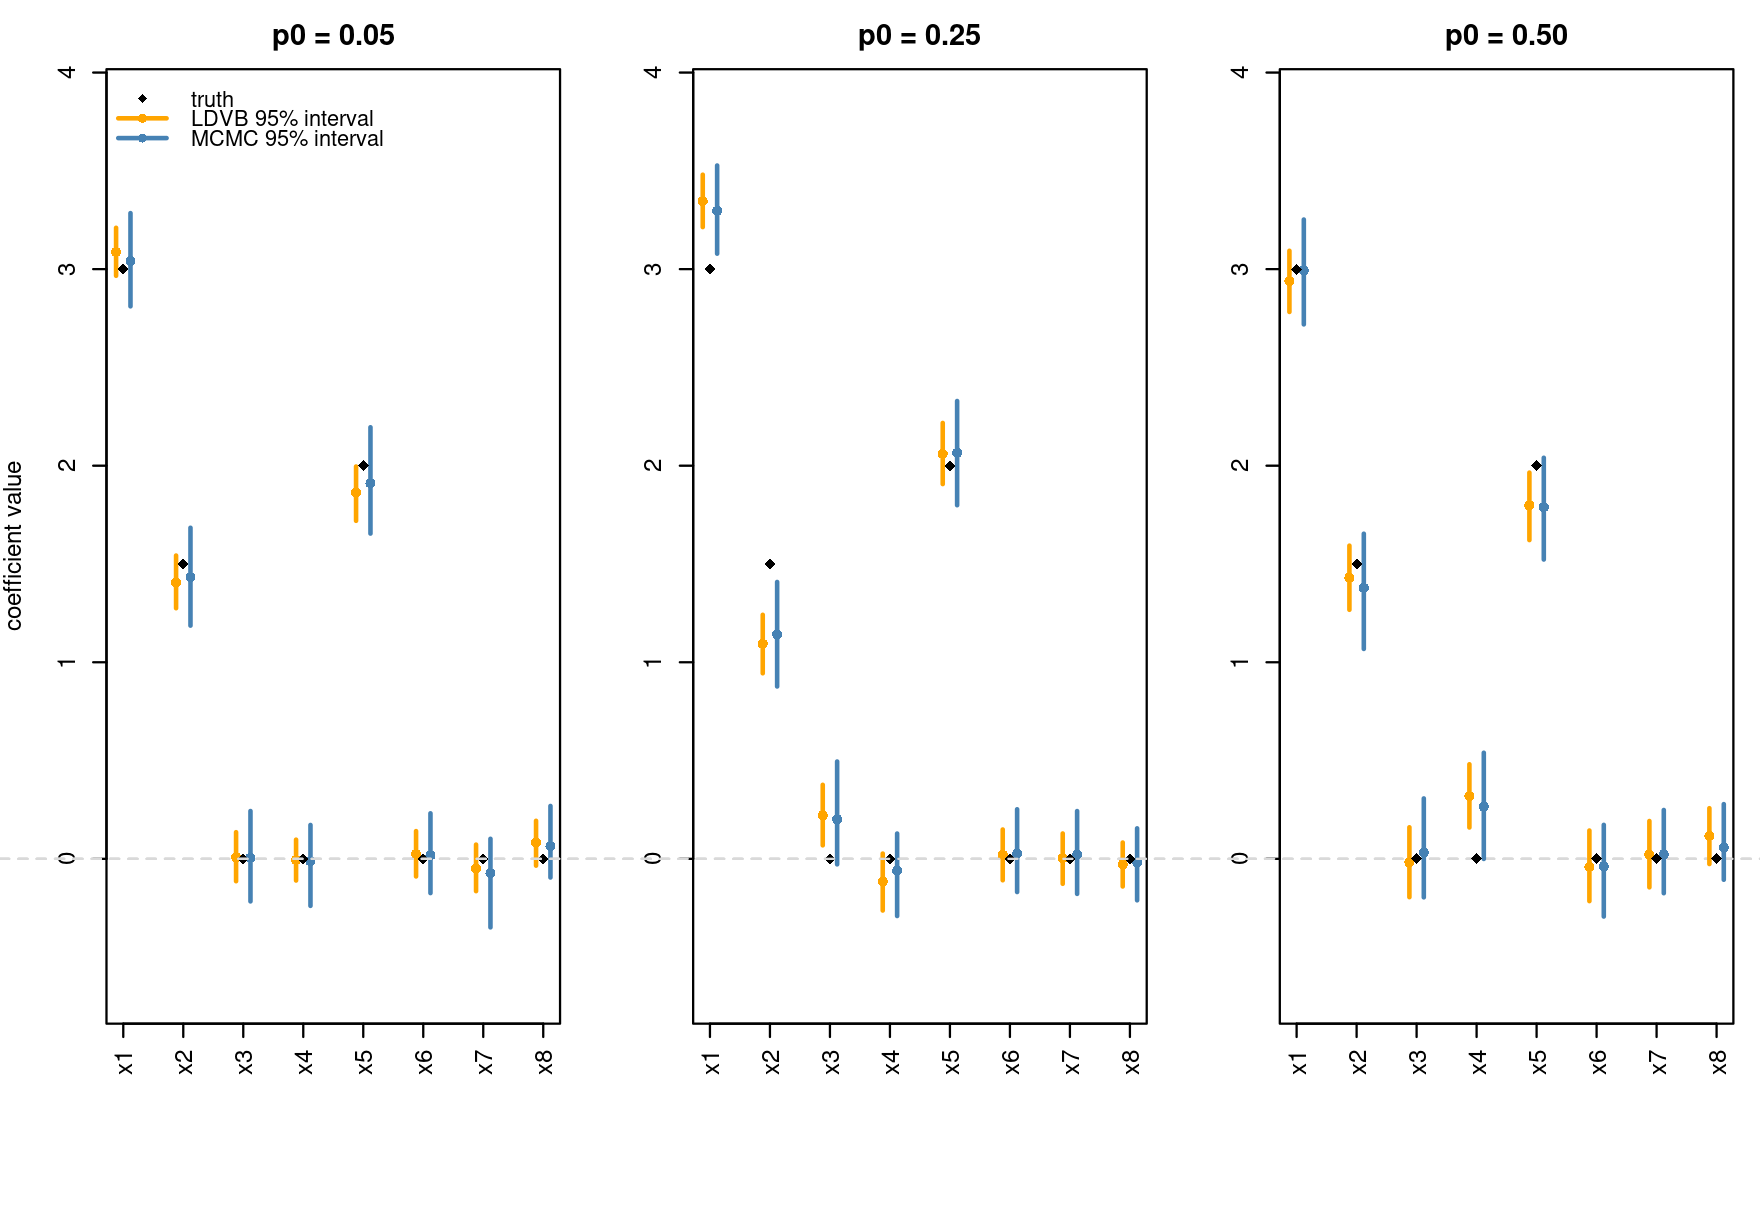
\includegraphics[width=0.95\textwidth]{figures/ch02-exdqlm/ex4static.png}
\caption[Sparse static exAL coefficient recovery]{Example 3: sparse static exAL regression under the correlated Gaussian benchmark with the \code{rhs\_ns} prior. Black diamonds denote the true non-intercept coefficients, orange intervals denote LDVB 95\% posterior intervals, and blue intervals denote MCMC 95\% posterior intervals. Panels correspond to \(p_0 = 0.05, 0.25,\) and \(0.50\).}
\label{exd:fig:ex4static}
\end{figure}

Figure \ref{exd:fig:ex4static} shows that, in this simulated realization, both methods recover the main sparse signal structure and shrink most null coefficients toward zero across the lower tail, lower-middle quantile, and median. Recovery is not uniform across coefficients: the smaller active coefficient is more difficult in the median fit, and a few null-coefficient intervals can miss zero. Across the three panels, the MCMC intervals give cleaner active-signal recovery in the two lower-tail fits, while the median fit is closer; the LDVB intervals provide a faster approximation to the same coefficient-level summaries.

\begin{table}[t!]
\centering
\TableStyle
{\setlength{\tabcolsep}{3pt}
\begin{tabular}{@{}llrrrr@{}}
 \toprule
 \(p_0\) & method & \shortstack{runtime\\(s)} & \shortstack{active\\RMSE} & \shortstack{null\\MAE} & \shortstack{holdout\\qRMSE} \\
 \midrule
 \tworowcell{0.05} & LDVB & \textbf{31.46} & 0.108 & \textbf{0.034} & 0.673 \\
 & MCMC & 71.92 & \textbf{0.069} & 0.035 & \textbf{0.594} \\
 \midrule
 \tworowcell{0.25} & LDVB & \textbf{27.74} & 0.310 & 0.078 & 0.371 \\
 & MCMC & 71.19 & \textbf{0.271} & \textbf{0.065} & \textbf{0.329} \\
 \midrule
\tworowcell{0.50} & LDVB & \textbf{12.66} & \textbf{0.128} & 0.103 & 0.341 \\
 & MCMC & 71.77 & 0.141 & \textbf{0.083} & \textbf{0.335} \\
 \bottomrule
\end{tabular}}
\caption[Sparse static exAL runtime and recovery metrics]{Example 3: runtime and sparse-signal recovery metrics for the static exAL fits under the \code{rhs\_ns} prior. The LDVB rows use \code{n.samp = 3000}, and the MCMC rows use 2000 burn-in iterations and 3000 retained draws. The active RMSE is computed over the three nonzero coefficients, the null MAE is computed over the five zero coefficients, and the holdout quantile RMSE is computed against the true target quantile on an independent holdout sample of size 800. Because the columns are the comparison metrics, bold entries indicate the smaller value within each quantile block; displayed ties are left unbolded.}
\label{exd:tab:ex4static}
\end{table}

The \code{exalStaticDiagnostic} objects returned by \code{diagnostics()} store the coefficient posterior summaries and holdout reference RMSEs used in Table \ref{exd:tab:ex4static}. Because the true coefficient vector is known in this simulation, the active-signal RMSE and null-coefficient MAE are computed directly from those coefficient summaries and the known truth.




The results reinforce the visual comparison in Figure \ref{exd:fig:ex4static}. The MCMC posterior-simulation fit has the smaller holdout quantile RMSE in all three fits, although the median difference is small. MCMC gives smaller active-signal RMSE at \(p_0 = 0.05\) and \(p_0 = 0.25\), while LDVB is slightly smaller at \(p_0 = 0.50\). Null-coefficient MAE is slightly smaller for LDVB at \(p_0 = 0.05\) and for MCMC at \(p_0 = 0.25\) and \(p_0 = 0.50\). The LDVB fit is nevertheless faster in all three cases, with runtime reductions of roughly 2.4-fold at \(p_0 = 0.05\), 2.4-fold at \(p_0 = 0.25\), and 6.1-fold at \(p_0 = 0.50\). In this benchmark, LDVB provides the lower-runtime approximation, whereas static MCMC supplies the posterior-simulation comparison used to examine interval and tail behavior.

\section{Chapter summary and limitations}
\label{exd:sec:summary}


The contribution of \pkg{exdqlm} is to make an established class of Bayesian
dynamic quantile models available through a coherent statistical interface and
to extend its computation. In particular, the package joins composable
state-space specification with MCMC, ISVB, and the later LDVB approximation;
standardizes summaries, diagnostics, prediction, and post-fit synthesis; and
adds static AL/exAL regression under shrinkage priors. The structured LDVB
factor retains conditional scale--skewness dependence and supplies a
deterministic alternative to the inherited importance-sampling approximation.

The three retained examples support different parts of this claim. Lake Huron
combines separate dynamic fits, multi-step forecasting, and synthesis of
posterior predictive draws. Sunspots compares DQLM and exDQLM fits and shows
the computational and predictive tradeoff between LDVB and MCMC: LDVB is
faster in the recorded fits, whereas MCMC gives smaller CRPS and PPLC. The
sparse simulation evaluates the static regularized-horseshoe routines under
a known conditional quantile; it likewise shows faster LDVB fitting but
generally smaller holdout quantile error under MCMC. These results establish
functionality and illustrate approximation tradeoffs, not a general predictive
advantage for one inferential method.

The scope remains deliberately bounded. Dynamic models are fitted one quantile
level at a time, and \code{quantileSynthesis()} combines predictive draws after
separate fits rather than defining a joint posterior across quantiles. LDVB
draws come from fitted variational factors, so MCMC remains the reference when
posterior tails or interval widths are central. Transfer-function decay is
fixed or grid-selected, and the reported runtimes apply only to the stated
hardware and fitting settings. Further work includes direct assessment of
variational approximation error, joint regularization across quantile levels,
nonlinear state evolution, and multivariate responses. Appendix
\ref{app:exdqlm-technical} records the nonstandard posterior calculations
needed to interpret the implemented procedures.
